\chapter{Architecture}
\label{chapter:architecture}

Alcaudon's architecture will be described in this chapter following a top-down
approach. Firstly, a general description of the different components of the system
will be explained. Finally, each of the components will be described more thoroughly.

\subsection{General description}

Alcaudon's platform is composed by 3 main units.

\begin{itemize}
\item \textbf{Alcaudon library}: This is the main interface between users
  and the system. In order to use Alcaudon it is necessary to have access to a
  cluster with a coordinator and computing nodes. This interface is provided as
  a library containing the tools to build dataflows, the interfaces to implement
  user defined stream computations and the tools to connect with a particular
  cluster. Since the computations are potentially infinite, the operations
  performed against the cluster are asynchronous, returning an id associated
  with the created operation.
\item \textbf{Coordinator node}: This is the main component of the system. It
  coordinates the life cycle of the different components of the cluster such as
  the computing nodes. It is also responsible of performing the scheduling of
  the user defined dataflows given the resources provided by the computing
  nodes. Finally, it is the interface between the cluster and the users, where
  they deploy their dataflow topologies.

\item \textbf{Computing nodes}: These nodes are in charge of executing the
  actual computations provided by Alcaudon's users. These nodes take care of
  storing intermediate results published to streams. They register dynamically
  to the cluster contacting the coordinator node. A deployment can be composed
  from one computing node up to thousands, as needed. Each of these nodes
  provides certain resources to the system, known as \textit{computation slots}.
  The number of slots is configurable, but they correlate with the number of
  available CPU's in the underlying hardware.
\end{itemize}

A high level overview of the system can be seen in
figure~\ref{fig:architecture}. The majority of the parts of the system have been
modeled as Actors. As it was stated previously it is a very good fit for this
kind of applications. Where possible, object oriented design patterns\cite{gof}
such as \textbf{builder} or \textbf{factory} have been used. However, functional
programming constructs such as monads\cite{monads}, type
classes\cite{typeclasses} or Algebraic Data Types have been used more widely.

Once the different parts of the system have been presented, they will be
inspected in detail.

\begin{figure}
  \centering
  \includegraphics[width=1\textwidth]{architecture.pdf}
  \caption{Alcaudon architecture schema}
  \label{fig:architecture}
\end{figure}

\subsection{Alcaudon library}

In the first place, the user facing interface will be presented in detail. In order
to create a streaming data processing pipeline, or dataflow topology as it has
been defined during all this document, users should provide their business
logic. To achieve this goal, Alcaudon provides certain interfaces so users
just need to care about their code. These interfaces are available as a library
that can be found at at Sonatype OSSRH \footnote{http://central.sonatype.org/pages/ossrh-guide.html}.

\begin{figure}
  \centering
  \includegraphics[width=0.6\textwidth]{client.pdf}
  \caption{Alcaudon library}
  \label{fig:library}
\end{figure}

This library is composed of three modules as it is shown in figure~\ref{fig:library}:

\begin{itemize}
\item Computation API's: Interface that users should implement in order to
  create computations.
\item Dataflow builder: This component is used to build dataflow topologies and
  later on submit the to the cluster coordinator.
\item Cluster client: Communication layer between clients and Alcaudon clusters.
  It handles all the operations needed to submit custom code to the cluster as well
  as the stream processing pipeline definition.
\end{itemize}

\subsubsection{Computation API's}

\begin{figure}[!h]
  \begin{center}
  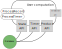
\includegraphics[width=0.5\textwidth]{libraryApi.pdf}
  \caption{Alcaudon computation API's}
  \label{fig:apis}
  \end{center}
\end{figure}

As explained before, in order to create custom computations to process unbounded
data-sets in Alcaudon, it is necessary to implement an interface. The interface
is listed in~\ref{code:computation}. This interface gives access to the
abstractions provided by the system as represented in figure~\ref{fig:apis}. As
it can be observed, there are two methods to be implemented;
\lstinline[columns=fixed]{def processRecord(record: Record): Unit} and \lstinline[columns=fixed]{def processTimer(timer: Timer): Unit}.

\begin{lstlisting}[language=scala, frame=trBL, label=code:computation, float=ht, caption = {Computation API's}]
trait Computation
    extends ProduceAPI
    with TimerAPI
    with StateAPI
    with SerializationAPI
    with RuntimeContext {
  ...
  def processRecord(record: Record): Unit
  def processTimer(timer: Timer): Unit
  ...
}
\end{lstlisting}

These methods represent the main entry point into user code, hooked in reaction to
record receipt and timers expiration. These constitute the application logic.
Within the execution of these methods, Alcaudon provides different functions to
work with persistent state, publish new records to streams, set timers or
serialize arbitrary data types. Those auxiliary API's are listed
in~\ref{code:auxiliaryComputations}. In Alcaudon, each computation can subscribe to
multiple sources represented as streams. Data travels in its simplest form,
as an array of bytes.

\begin{figure}
  \begin{center}
    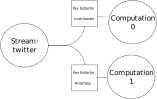
\includegraphics[width=0.5\textwidth]{keypartitioning.pdf}
    \caption{Alcaudon record key assignment}
    \label{fig:keypartitioning}
  \end{center}
\end{figure}

However, for each stream subscription users should provide
a key extraction function, this process can be shown in figure
~\ref{fig:keypartitioning}. Having a key per record allows the implementation of
parallelization strategies such as key partitioning. Therefor, every record
emitted by one of the subscribed sources, an instance of the class
\lstinline[columns=fixed]{Record} listed in ~\ref{code:records} will be
injected with the call to \lstinline[columns=fixed]{processRecord}.

\begin{lstlisting}[language=scala, frame=trBL, label=code:records, float=ht, caption = {Record classes}]
case class RawRecord(value: Array[Byte], timestamp: Long) {
  val id = UUID.randomUUID().toString
}
case class Record(key: String, rawRecord: RawRecord) {
  val value = rawRecord.value
  val timestamp = rawRecord.timestamp
  val id = UUID.randomUUID().toString
}
\end{lstlisting}

Timers are the other possible trigger for user defined code execution. In
Alcaudon there are three types of timers:

\begin{itemize}
\item \textit{Fixed timers}: This kind of timers are triggered once at a
  specific wall time.
\item \textit{Recurrent fixed timers}: This timer is just like the previous
  timers, however it is executed recurrently. I.E., every five minutes.
\item \textit{Watermark timers}: This timer try to estimate the point where all
  the events up to certain window have been consumed by the system and execute
  then. The mechanism and algorithm used to implement them will be explained
  later.
\end{itemize}

When a timer is executed it has as a parameter an instance of the class Timer
listed in ~\ref{code:timers}. This constructs are key to the domain of unbounded
data-sets due to its very nature. A mean to emit partial results is needed, so
this is the mechanism provided by Alcaudon to emit results.

\begin{lstlisting}[language=scala, frame=trBL, label=code:timers, float=ht, caption = {Timer class}]
  case class Timer(tag: String, timestamp: Long)
\end{lstlisting}

\subsubsection{Dataflow builder}

Once the computations are implemented, users need a way to build the dataflow topologies.
To achieve this goal, the system provides a dataflow builder. Using this instrument,
users are able to define dependencies among the computations in the system.
These main entities that can be used in Alcaudon are:

\begin{itemize}
  \item \textit{Sources}: Sources bring external data into the system. Some
    examples could be a TCP/IP socket, Twitter streaming API, Apache Kafka,
    Zeromq, etc.
  \item \textit{Computations}: Computations are user defined business logic.
  \item \textit{Streams}: Streams represent the delivery instrument between
    different computations in Alcaudon. Computations subscribe to one or more
    streams and publish to zero or more streams. Alcaudon guarantees the
    delivery of records along these streams.
  \item \textit{Sinks}: Sinks are an special kind of streams, providing a way to
    publish data to external systems such as http endpoints or databases. They
    are useful to project final results.
\end{itemize}

Alcaudon dataflow builder is defined in listing~\ref{code:builder}. Dependencies
are checked, thus if one computation depends or publish into an unknown stream,
the dataflow definition will be considered invalid. Internally, defined
dataflows are represented as a directed acyclic graph. In this graph, vertices
represent computations and streams while edges represent the dependencies
between them or how data flow along the system. Considering that the execution
of the dataflow is performed remotely and computations are arbitrary user code,
computations are represented as its fully qualified name inside the JVM
classpath. Using this fully qualified name in combination with dynamic class
loaders it is possible to load code dynamically. In conclusion, with this builder
it is possible to create a declarative representations of Alcaudon data pipelines.
This representation abstracts away all the details about in which compute nodes
code will run or how parallelism will be implemented. This approach is quite
similar to how Free Monad\cite{freemonad}, SQL or Prolog works.

\begin{lstlisting}[language=scala, frame=trBL, label=code:builder, float=ht, caption = {Alcaudon's DataflowBuilder}]
DataflowBuilder(dataflowName: String)
  .withSource(sourceName: String, sourceDescription: SourceDescription)
  .withComputation(computationName: String,
    computation: Computation,
    outputStreams: Set[StreamID],
    AlcaudonInputStream(StreamID)(keyExtractor: Array[Byte] => String)*
  .withSink(sinkName: String, sinkDescription: SinkDescription)
  .build()
\end{lstlisting}

\subsubsection{Cluster client}

\begin{figure}
  \centering
  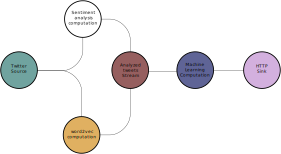
\includegraphics[width=0.8\textwidth]{dataflowbuilder.pdf}
  \caption{Dataflow example}
  \label{fig:dataflowbuilder}
\end{figure}

Once the computations and topology have been defined as in
figure~\ref{fig:dataflowbuilder}, it is needed to have some machinery in order
to execute them in an Alcaudon cluster. In Alcaudon library there are the tools
needed to connect to an existing cluster and perform certain operations. The
available operations are listed in table~\ref{tab:operations}. Creating a
dataflow pipeline is an asynchronous operation, returning a DataflowPipeline
\acf{UUID} that identifies the created pipeline. With this \acs{UUID} it is
possible to perform some operations over the pipeline.

\begin{table}[hp]
\centering
\begin{tabular}{|l|l|l|}
\hline
\textbf{Action} & \textbf{Parameters} & \textbf{Returned info} \\ \hline
\begin{tabular}[c]{@{}l@{}}Send Dataflow topology\end{tabular}  & DataflowGraph and user JAR's & DataflowPipeline UUID \\ \hline
\begin{tabular}[c]{@{}l@{}}Get DataflowJob execution info\end{tabular} & DataflowPipeline UUID & DatflowPipelineStatus \\ \hline
\begin{tabular}[c]{@{}l@{}}Stop DataflowJob execution\end{tabular} & DataflowPipeline UUID & DatflowPipelineStatus \\ \hline
\end{tabular}
\caption{Available cluster management operations}
\label{tab:operations}
\end{table}

In order to understand better how Alacaudon dataflow pipeline creation works, it
will be explained more thoroughly. This operation is divided into two phases,
first user code libraries are uploaded. Once the libraries are uploaded the
actual dataflow pipeline is created. Uploading user libraries is needed so
computing nodes can have access to user business logic. The number of computing nodes that
can access concurrently to these user libraries depends on the deployment,
reaching up to thousands in some cases. To avoid any scaling problems, libraries
are stored into an object storage service. In this case, they are stored in
Amazon S3\footnote{https://aws.amazon.com/s3/}. These services usually provide a
way to avoid the need to first upload the data to a backend server in order to
get access to credentials to later on upload data to an object storage services.
This is achieved using pre-signed URL's, based on a temporary token generated
using service credentials and a timestamp. In Alcaudon, cluster clients
request the creation of a dataflow pipeline. As a response, a pre-signed URL
alongside an UUID that identifies the operation is returned by the cluster
coordinator. Once cluster clients have the URL, they can use it to upload user
code directly to the object storage service. With the user code uploaded, the
next step is to create the actual Dataflow pipeline. Given the returned UUID a
request is done to cluster coordinator in order to finish the dataflow pipeline
creation. The communication is performed using akka-remote that allows
communicate with remote actor systems.The whole process is represented as a
sequence diagram in figure~\ref{fig:pipelinecreation}. This process is performed
transparently by the library from users perspective.

\begin{figure}[!h]
\begin{center}
\includegraphics[width=0.8\textwidth]{dataflowcreation.png}
\caption{Sequence diagram for Dataflow pipeline creation}
\label{fig:pipelinecreation}
\end{center}
\end{figure}

\subsubsection{Serialization API}

Programmers are used to work with high level abstractions in order to model the
domain they are working on. As it has been described previously, records in
Alcaudon are a tuple of a key and an array of bytes. Given this fact, a way to
work with high level entities is needed. There are many options to serialize and
deserialize data available, such as JSON, Protocol Buffers, etc. Alcaudon users
are free to use the serialization format that they prefer but to ease to work
with the platform, a generic serialization library typeclass is provided. This
library is capable of, given an \acs{ADT} generate automatically serializers and
deserializers during compile time. This is possible thanks to an advance Scala
feature, implicits resolution, and one library for generic programming,
Shapeless. \acs{ADT}'s are a functional programming concept that allow data
representation in terms of \textit{products} and \textit{sums} of types. A
\textit{product} is a combination of different types $(A \& B)$, on the other
hand a \textit{sum} is an alternation of different types $(A | B)$. In Scala,
\acs{ADT} are expressed as case classes and traits as shown in
listing~\ref{code:adt}.

\begin{lstlisting}[language=scala, frame=trBL, label=code:adt, float=ht, caption = {\acs{ADT} example}]
  sealed trait Message // Message = (Tweet | Account)
  case class Tweet(user: String, text: String, timestamp: Long) extend Message // Tweet = (String & String & Long)
  case class Account(name: String, age: Int) extend Message // Account = (String & Int)
\end{lstlisting}

Taking this into account, case classes could be represented as lists of types,
in \lstinline[columns=fixed]{Tweet} example it can be summarized as a list of
three types, \lstinline[columns=fixed]{String & String & Long}. Shapeless allows
to represent case classes as a heterogeneous lists of types and work with them
as they are regular types. Once it is possible to encode \acs{ADT}'s as
heterogeneous lists of types a tool to convert that generic representation into
a serializer is needed. To achieve this goal, Scala implicit type system is the
answer. Scala implicits are a way to provide certain parameters marked as
implicits to functions without the need to pass them explicitly. Scala compiler has
a set of strict rules\footnote{http://docs.scala-lang.org/tutorials/FAQ/finding-implicits.html}
to look for implicit parameters. The interesting part comes when functions with implicit
parameters use parametric polymorphism, such as Alcaudon's serialization typeclass
listed in~\ref{code:typeclass}.
\begin{lstlisting}[language=scala, frame=trBL, label=code:typeclass, float=ht, caption = {Serializer Deserializer typeclass}]
trait TypeInfo[T] {
  def serialize(obj: T)(implicit output: DataOutput): DataOutput
  def deserialize(t: DataInput): T
}
\end{lstlisting}

It is possible to write a rule that creates a \lstinline[columns=fixed]{TypeInfo} for $(A, B)$ given
\lstinline[columns=fixed]{TypeInfo} for $A$ and $B$. This feature is provided by Scala implicit resolution
mechanism that works as an inductive solver.

\begin{lstlisting}[language=scala, frame=trBL, label=code:typeclass, float=ht, caption = {Serializer Deserializer typeclass}]
  implicit def genericObjectEncoder[A, H <: HList, O <: HList](
      implicit generic: LabelledGeneric.Aux[A, H],
      repFormat: Lazy[TypeInfo[H]],
      keys: Keys.Aux[H, O],
      ktl: ToList[O, Any]
  ): TypeInfo[A] =
    new TypeInfo[A] {
      def serialize(v: A)(implicit output: DataOutput) = {
        repFormat.value.serialize(generic.to(v))
      }

      def deserialize(input: DataInput) = {
        generic.from(repFormat.value.deserialize(input))
      }
    }

  implicit def hListFormat[Key <: Symbol, Value, Remaining <: HList](
      implicit key: Witness.Aux[Key],
      lazyTih: Lazy[TypeInfo[Value]],
      lazyTit: Lazy[TypeInfo[Remaining]]
  ): TypeInfo[FieldType[Key, Value] :: Remaining] =
    new TypeInfo[FieldType[Key, Value] :: Remaining] {

      val tih = lazyTih.value
      val tit = lazyTit.value

      def serialize(hlist: FieldType[Key, Value] :: Remaining)(
          implicit output: DataOutput) = {
        val headOutput = tih.serialize(hlist.head)
        tit.serialize(hlist.tail)(headOutput)
      }

      def deserialize(input: DataInput) = {
        val head = tih.deserialize(input)
        val tail = tit.deserialize(input)
        field[Key](head) :: tail
      }

    }

    ...
    ...
  implicit object LongTypeInfo extends TypeInfo[Long] {
    def serialize(t: Long)(implicit output: DataOutput): DataOutput = ...
    def deserialize(t: DataInput): Long = ...
  }
  implicit object FloatTypeInfo extends TypeInfo[Float] {
    def serialize(t: Float)(implicit output: DataOutput): DataOutput = ...
    def deserialize(t: DataInput): Float = ...
  }
\end{lstlisting}

\subsection{Coordinator node}
\lipsum

\subsection{Computation node}
\lipsum
